\documentclass{article}

\usepackage{graphicx}
\usepackage{tikz}
\usepackage{tikzsymbols}
\usetikzlibrary{calc,patterns,shapes.geometric}
\pagestyle{empty}
\usepackage[margin=0pt]{geometry}
\geometry{papersize={14in,12in}}

\def\centerarc[#1](#2)(#3:#4:#5){\draw[#1] ($(#2)+({#5*cos(#3)},{#5*sin(#3)})$) arc (#3:#4:#5);}

\begin{document}
	\begin{figure}
		\centering
		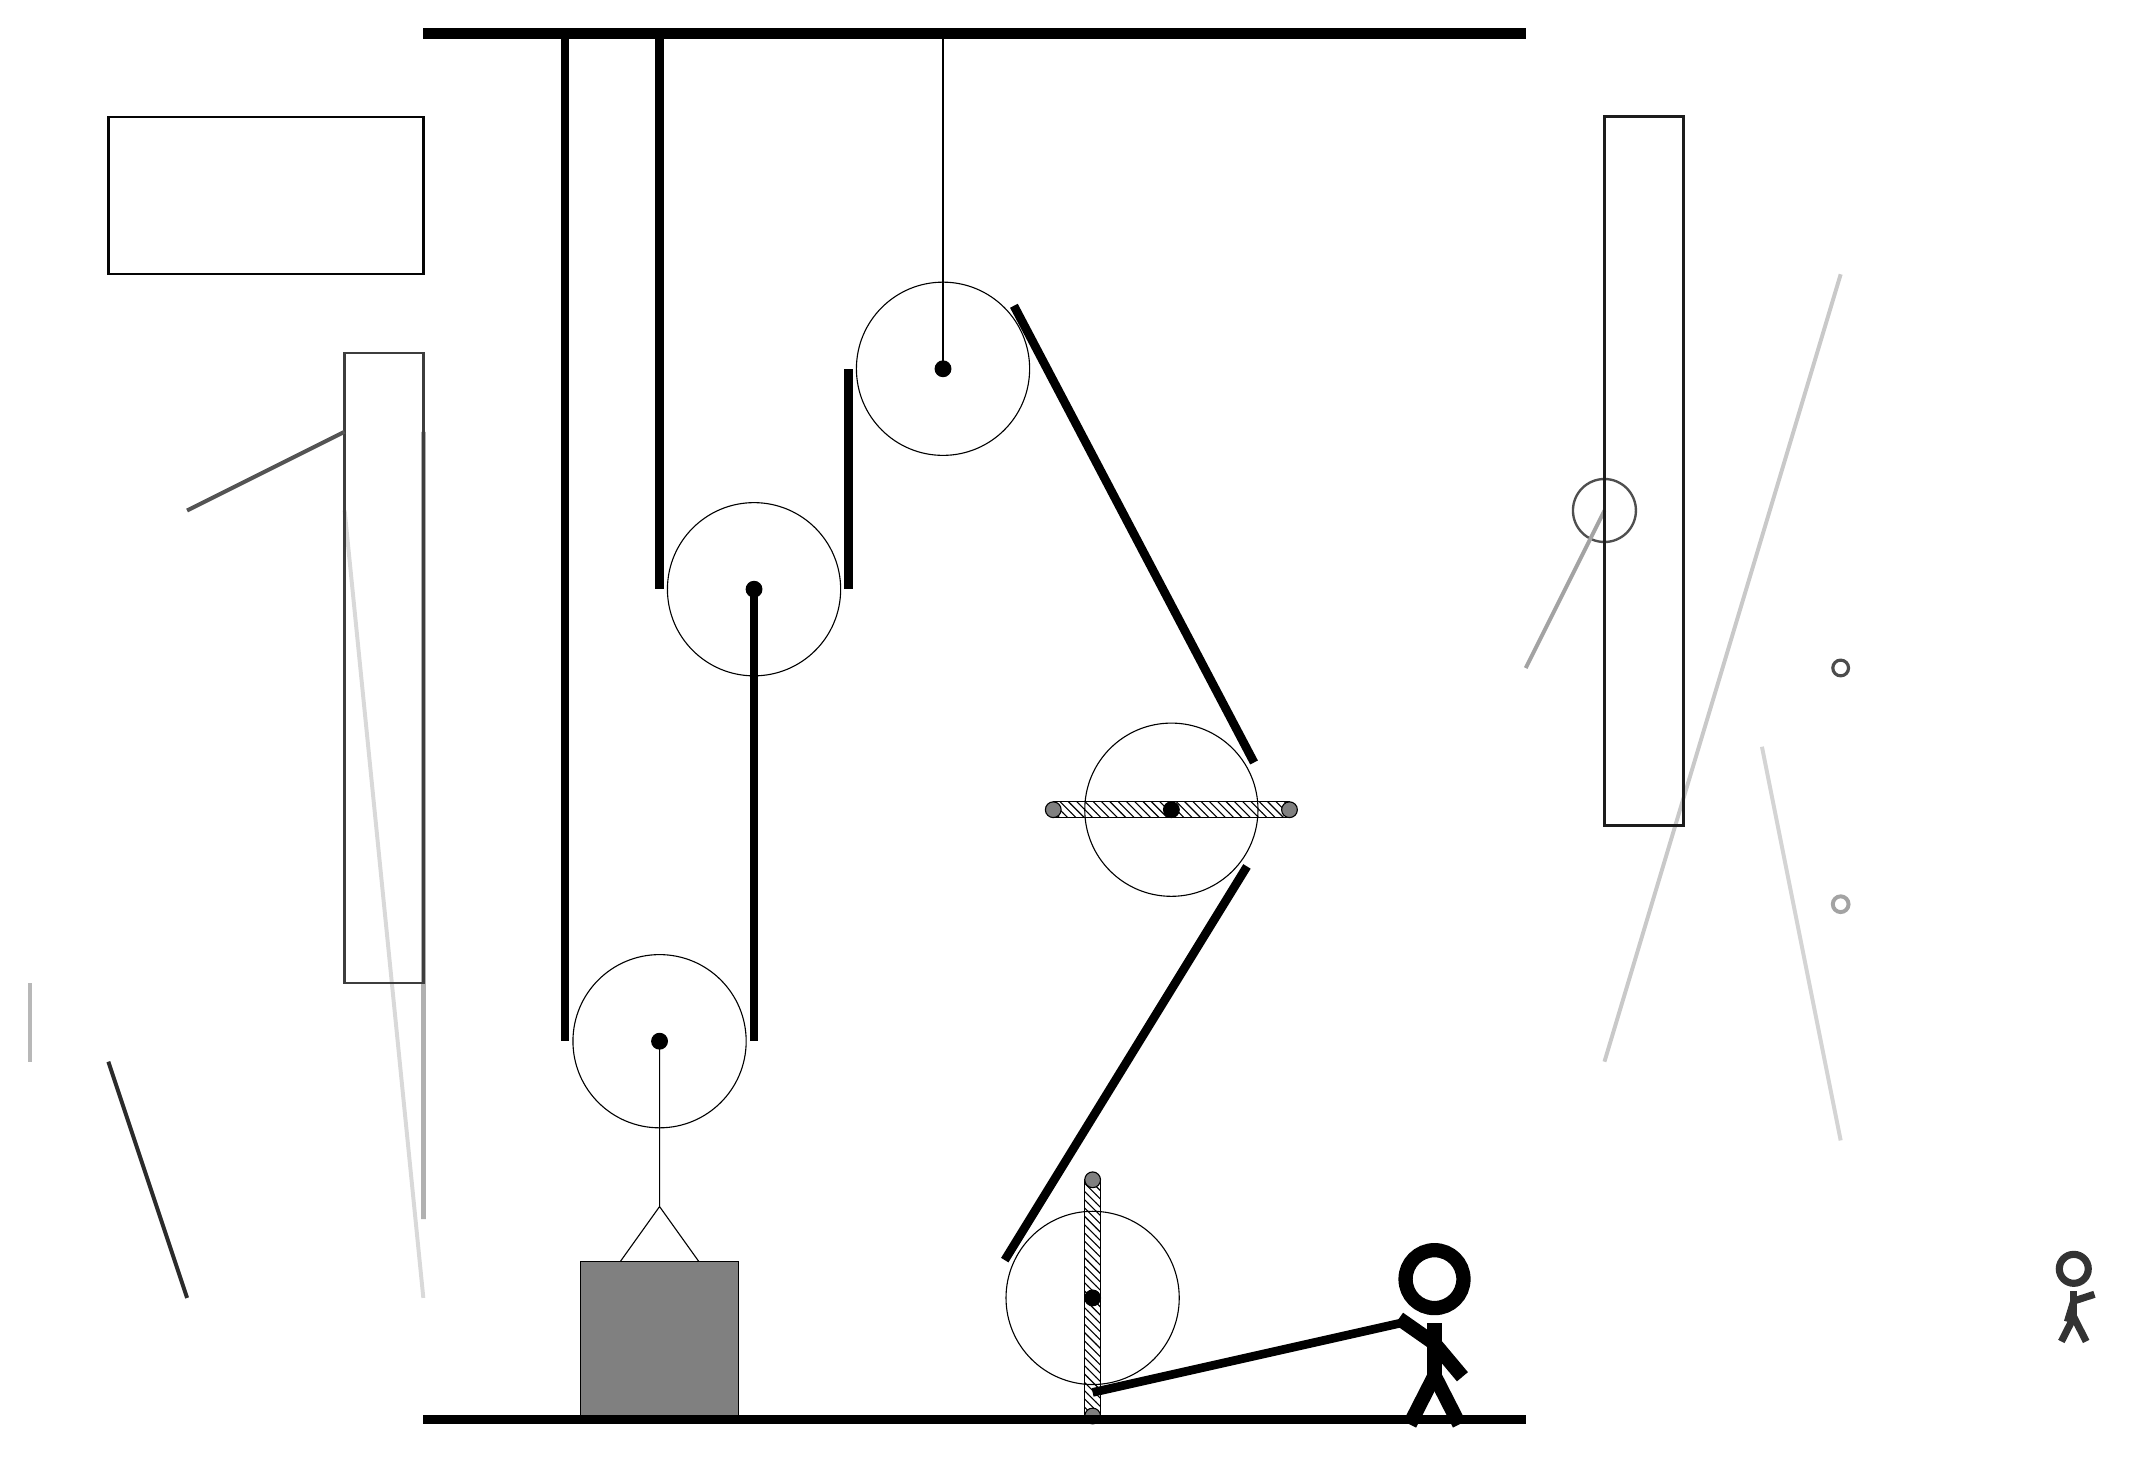
\begin{tikzpicture}
			%%%%% START %%%%%
			
			\draw[fill=black] (-2, 14) rectangle (12, 14.125);
			
			\draw (1, 1.26) circle (1.1);
			\draw[fill=black] (1, 1.26) circle (0.1);
			
			\draw (2.2, 7.0) circle (1.1);
			\draw[fill=black] (2.2, 7.0) circle (0.1);
			
			\draw (4.6, 9.8) circle (1.1);
			\draw[fill=black] (4.6, 9.8) circle (0.1);
			\draw[thick] (4.6, 9.8) -- (4.6, 14);
			
			\draw (6.5, -2) circle (1.1);
			\draw[fill=black] (6.5, -2) circle (0.1);
			\draw[pattern=north west lines, pattern color=black] (6.4, -0.5) rectangle (6.6, -3.5);
			\draw[fill=black!50] (6.5, -0.5) circle (0.1);
			\draw[fill=black!50] (6.5, -3.5) circle (0.1);
			
			\draw (7.5, 4.2) circle (1.1);
			\draw[fill=black] (7.5, 4.2) circle (0.1);
			\draw[pattern=north west lines, pattern color=black] (6.0, 4.3) rectangle (9.0, 4.1);
			\draw[fill=black!50] (6.0, 4.2) circle (0.1);
			\draw[fill=black!50] (9.0, 4.2) circle (0.1);
			
			\draw (1, 1.26) -- (1, -0.84) -- (0.5, -1.54) -- (1.5, -1.54) -- (1, -0.84);
			\draw[fill=black!50] (0, -1.54) rectangle (2, -3.54);
			
			\draw [line width=0.3mm, color=black!69](13, 8) circle (0.4);
			
			\draw[line width=0.5mm, color=black!36](13, 8) -- (12, 6);
			\draw[line width=0.5mm, color=black!21](16, 11) -- (13, 1);
			\draw[line width=0.5mm, color=black!15](-2, -2) -- (-3, 8);
			\draw[line width=0.5mm, color=black!17](15, 5) -- (16, 0);
			\draw[line width=0.3mm, color=black!98] (-2, 13) rectangle (-6, 11);
			\draw[line width=0.5mm, color=black!28](-7, 1) -- (-7, 2);
			\draw[line width=0.4mm, color=black!89] (13, 4) rectangle (14, 13);
			\draw [line width=0.4mm, color=black!70](16, 6) circle (0.1);
			\draw[line width=0.7mm, color=black!31] (-2, -1) rectangle (-2, 9);
			\draw[line width=0.3mm, color=black!76] (-3, 2) rectangle (-2, 10);
			
			\draw [line width=0.5mm, color=black!36](16, 3) circle (0.1);
			\node[line width=0.3mm, color=black!80] at (19, -2) {\Strichmaxerl[5][73][18]};
			\draw[line width=0.5mm, color=black!83](-6, 1) -- (-5, -2);
			\draw[line width=0.5mm, color=black!67](-3, 9) -- (-5, 8);
			\draw [line width=0.4mm, color=black!17](16, 7) circle (0.0);
			
			\draw[line width=1.1mm] (-0.2, 14) -- (-0.2, 1.26);
			\centerarc[line width=1.1mm](1, 1.26)(180:360:1.2000000000000002);
			\draw[line width=1.1mm](2.2, 1.26) -- (2.2, 7.0);
			\draw[line width=1.1mm] (1.0, 14) -- (1.0, 7.0);
			\centerarc[line width=1.1mm](2.2, 7.0)(180:360:1.2000000000000002);
			\draw[line width=1.1mm](3.4, 7.0) -- (3.4, 9.8);
			\centerarc[line width=1.1mm](4.6, 9.8)(35:180:1.2000000000000002);
			\draw[line width=1.1mm] (5.5, 10.6) -- (8.55, 4.8);
			\centerarc[line width=1.1mm](7.5, 4.2)(215:135:-1.2000000000000002);
			\draw[line width=1.1mm](8.46, 3.48) -- (5.384, -1.52);
			\centerarc[line width=1.1mm](6.5, -2)(-30:100:-1.2000000000000002);
			\draw[line width=1.1mm](6.5, -3.2) -- (10.5, -2.3);
			
			\node at (10.8, -2.5) {\Strichmaxerl[10][-35][-50]};
			
			\draw[fill=black] (-2, -3.5) rectangle (12, -3.6);
			
			%%%%% END %%%%%
		\end{tikzpicture}
	\end{figure}	
\end{document}